\documentclass[11pt,a4paper,final]{article}
\usepackage[utf8]{inputenc}
\usepackage{amsmath}
\usepackage{amsfonts}
\usepackage{amssymb}
\usepackage{float}
\usepackage{lipsum}
\usepackage{graphicx}
\usepackage{hyperref}

\begin{document}
\author{Adam Ingwersen, Peter Friborg, Aske Fjellerup}
\title{Ugeopgave 1 \\ PoP E16 \\ DIKU}
\maketitle

\section*{Introduktion}
I denne rapport præsenteres gruppens initielle opdagelser og løste opgaver i klik-og-peg programmeringssproget 'Scratch'. 

\section*{Del 1.1}
I denne delopgave er gruppen begrænset til at anvende 10 specifikke kodeblokke i 'Scratch'. 

\paragraph{-}
Først betragtes de 10 kodeblokke, som må anvendes til denne opgave. Det besluttes, at gruppen vil forsøge at anvende samtlige kodeblokke med det formål at skrive et program, der vil få programmets 'Sprite' til at gemme sig, hoppe frem og 'forskrække' spilleren. 

\begin{figure}[H]
\centering
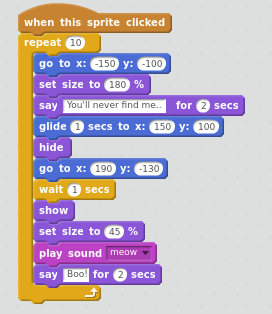
\includegraphics[scale = 0.4]{1_1.png}
\caption{Scratch program til delopgave 1.1}
\end{figure}

\pagebreak
\section*{Del 1.2}
Formålet i denne delopgave er at "designe \& implimentere et spil efter eget valg". Det er acceptabelt at bruge alle blokke der findes i 'Scratch'. \linebreak
\linebreak
Første trin i designfasen består af en mindstorm, der ender ud i at gruppen ville bestræbe sig på at lave en ny version af 'Fiskespillet'. Gameplayet i 'Fiskespillet' er, at man starter som en lille fisk og spiser mindre fisk for at blive større ved at bruge piletasterne. 
Med dette i mente: satte gruppen sig ved computeren og begyndte at designe et spil, med 'Sprite'en' 'Squirrel' som hovedfigur. 

\subsection*{Bevægelse af Sprite}
Spriten skal bevæge sig op/ned samt højre/venstre ved brug af piletasterne. En glidende funktion i scratch er her ikke hensigtsmæssig, da denne introducerer en forsinkelse for spilleren. Af denne årsag, valgte gruppen at anvende 'change-by' funktionen, som muliggør bevælgese relativt til Spritens nuværende position. For at berøringen tæller, skal spilleren bevæge spriten - dette sikrer, at spillet ikke kan gennemføres, hvis spilleren er inaktiv.  Kodeblokkene, der muliggør denne mekanisme er vist i 'Figure 2' nedenfor.

\begin{figure}[H]
\centering
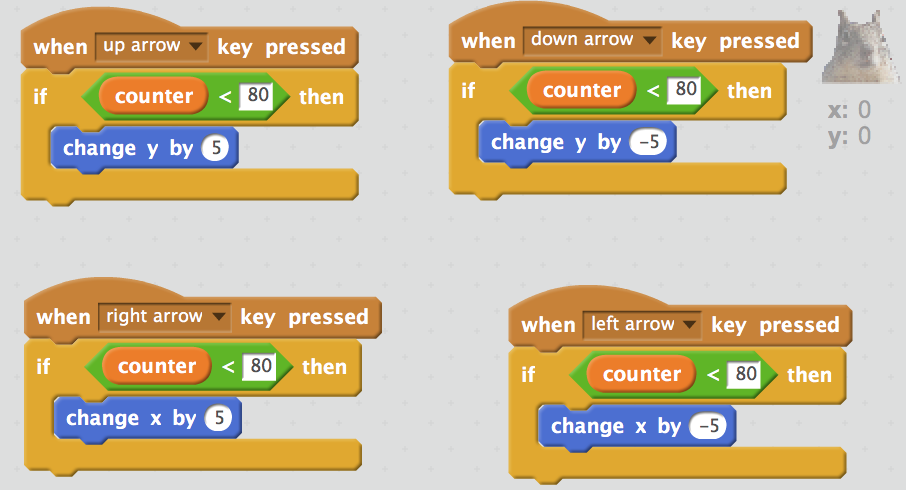
\includegraphics[scale = 0.4]{MovementSquirrel.png}
\caption{Squirrel bevægelses kode}
\end{figure}

\subsubsection*{Progression}

Egernet skal indsamle andre objekter, og ved berøring printes en passende besked. Spillet fortsætter ved at Squirrel-spriten aktiverer en tæller(counter) for hver berørt taco - og herefter vokser egernet marginalt i størrelse.


\subsection*{Bevægelse af andre objekter}

Vi ønskede, at Spriten skulle være i stand til at 'fange' andre objekter og dermed vokse for ultimativt at afslutte spillet. Til dette formål valgte vi 'Taco'-spriten. 
Taco-sprite(-rne) bevæger sig tilfældigt henover skærmen og når en taco berøres af Squirrel-spriten, reagerer disse ved at udsende en besked og forsvinde for derefter at dukke op et nyt, tilfældigt sted på skærmen og fortsætte som før, indtil endnu en berøring. 

\begin{figure}[H]
\centering
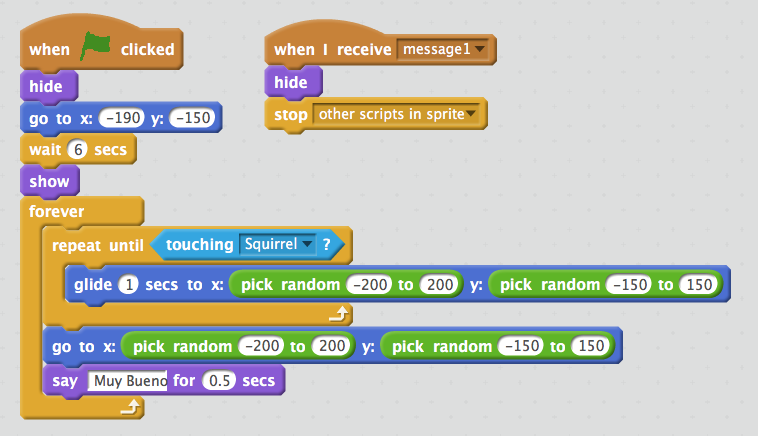
\includegraphics[scale = 0.4]{Tacos.png}
\caption{Tacos movement}
\end{figure}


\subsection*{Afslutning af spillet}

Egernet samt tacos fortsætter som anført ved at loope henover instruktionere, indtil spilslut opnås. 

Spillet er, pr. konstruktion, forholdsvist repetitivt, hvorved vi valgte at afslutte spillet ved 80 indsamlede tacos.
Når counteren når 80, vil Squirrel-spriten broadcaste en besked. Den samlede kode er anført i bilag 1. Den afsluttende del af spillet forløber som anført nedenfor:

\begin{enumerate}
\item{Gem og deaktiver Taco-sprites}
\item{Stop styring via piletaster}
\item{Få egernet til at printe besked for at indikere, at spillet aflsuttes}
\item{Flyt egern mod skærmens centrum}
\item{Lad solbriller glide ned over skærmen, således at egernet ved slut er påført solbriller}
\item{Slut ved at egernet printer en sidste besked}
\end{enumerate}

Spillet afsluttes med slutskærmen:

\begin{figure}[H]
\centering
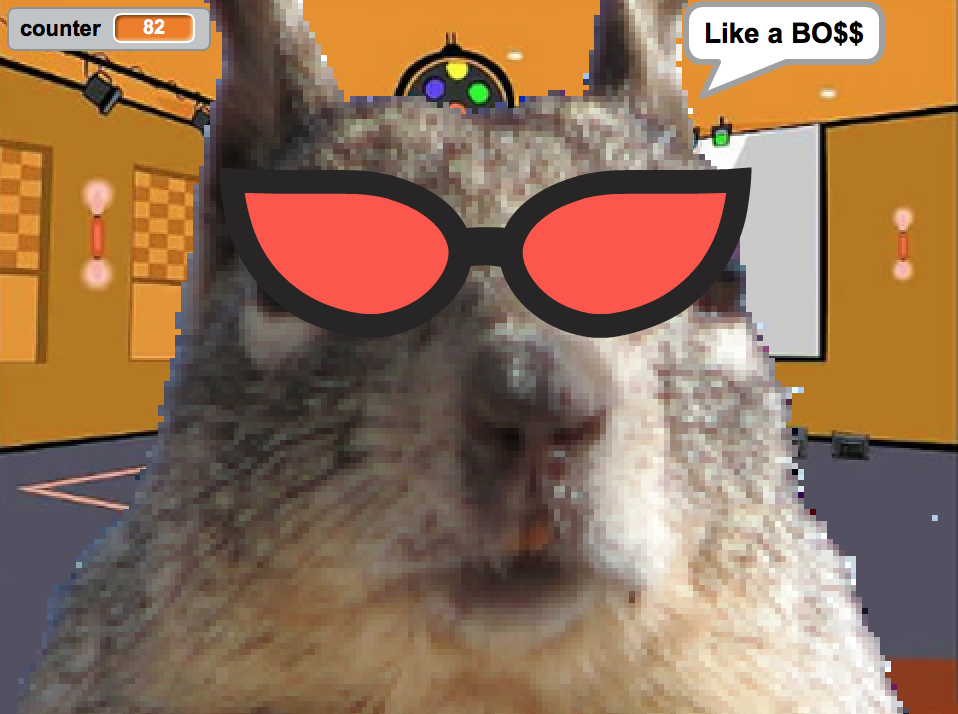
\includegraphics[scale = 0.4]{FatBossSquirrel.png}
\caption{Spils afslutning}
\end{figure}

\section*{Løbende forbedringer}

I takt med at spillet udformede sig, løb vi ind i en række problemer - disse blev løst ved følgende work-arounds:

\begin{enumerate}
\item{Problem: Taco's aktiverede stadigvæk egernet efter slut}
\begin{itemize}
\item{Løsning: Anvend 'Hide' + 'Stop(Other scripts in sprite)' sammen med broadcast-reaktionen}
\end{itemize}
\item{Problem: 'Wait until' [counter] '=' (80) reusulterede i, at spillet ikke sluttede, hvis egernet berørte 80'ende og 81'ende taco samtidigt}
\begin{itemize}
\item{Løsning: 'Wait until' [counter] 'larger than' (79)}
\end{itemize}
\item{Problem: Solbriller falder om bagved egern ved spil-slut}
\begin{itemize}
\item{Løsning: 'Go to front' ved aktivering via broadcast}
\end{itemize}
\end{enumerate}

\pagebreak
\section*{Bilag 1}
\begin{figure}[H]
\centering
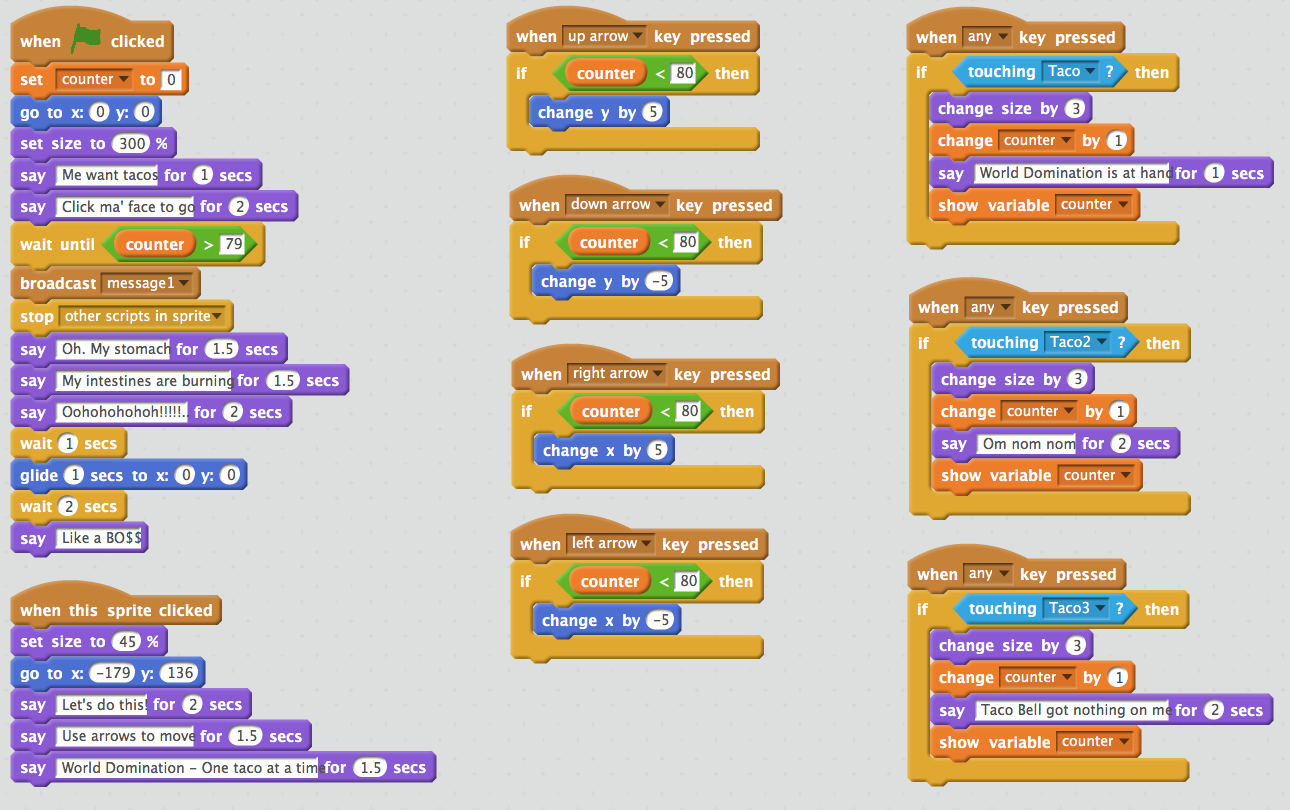
\includegraphics[scale = 0.4]{FullSquirrel.png}
\caption{Squirrels fulde Scratch kode}
\end{figure}

\subsection*{Link til program 1.1 \& Spil 1.2}
\begin{enumerate}
\item{\href{https://scratch.mit.edu/projects/120074250/}{Program 1}}
\item{\href{https://scratch.mit.edu/projects/120075655/}{Program 2}}
\end{enumerate}


\end{document}